
\chapter{Formas de onda} % Título del Anexo

\label{wave} 

\begin{figure}[h!]
    \centering
    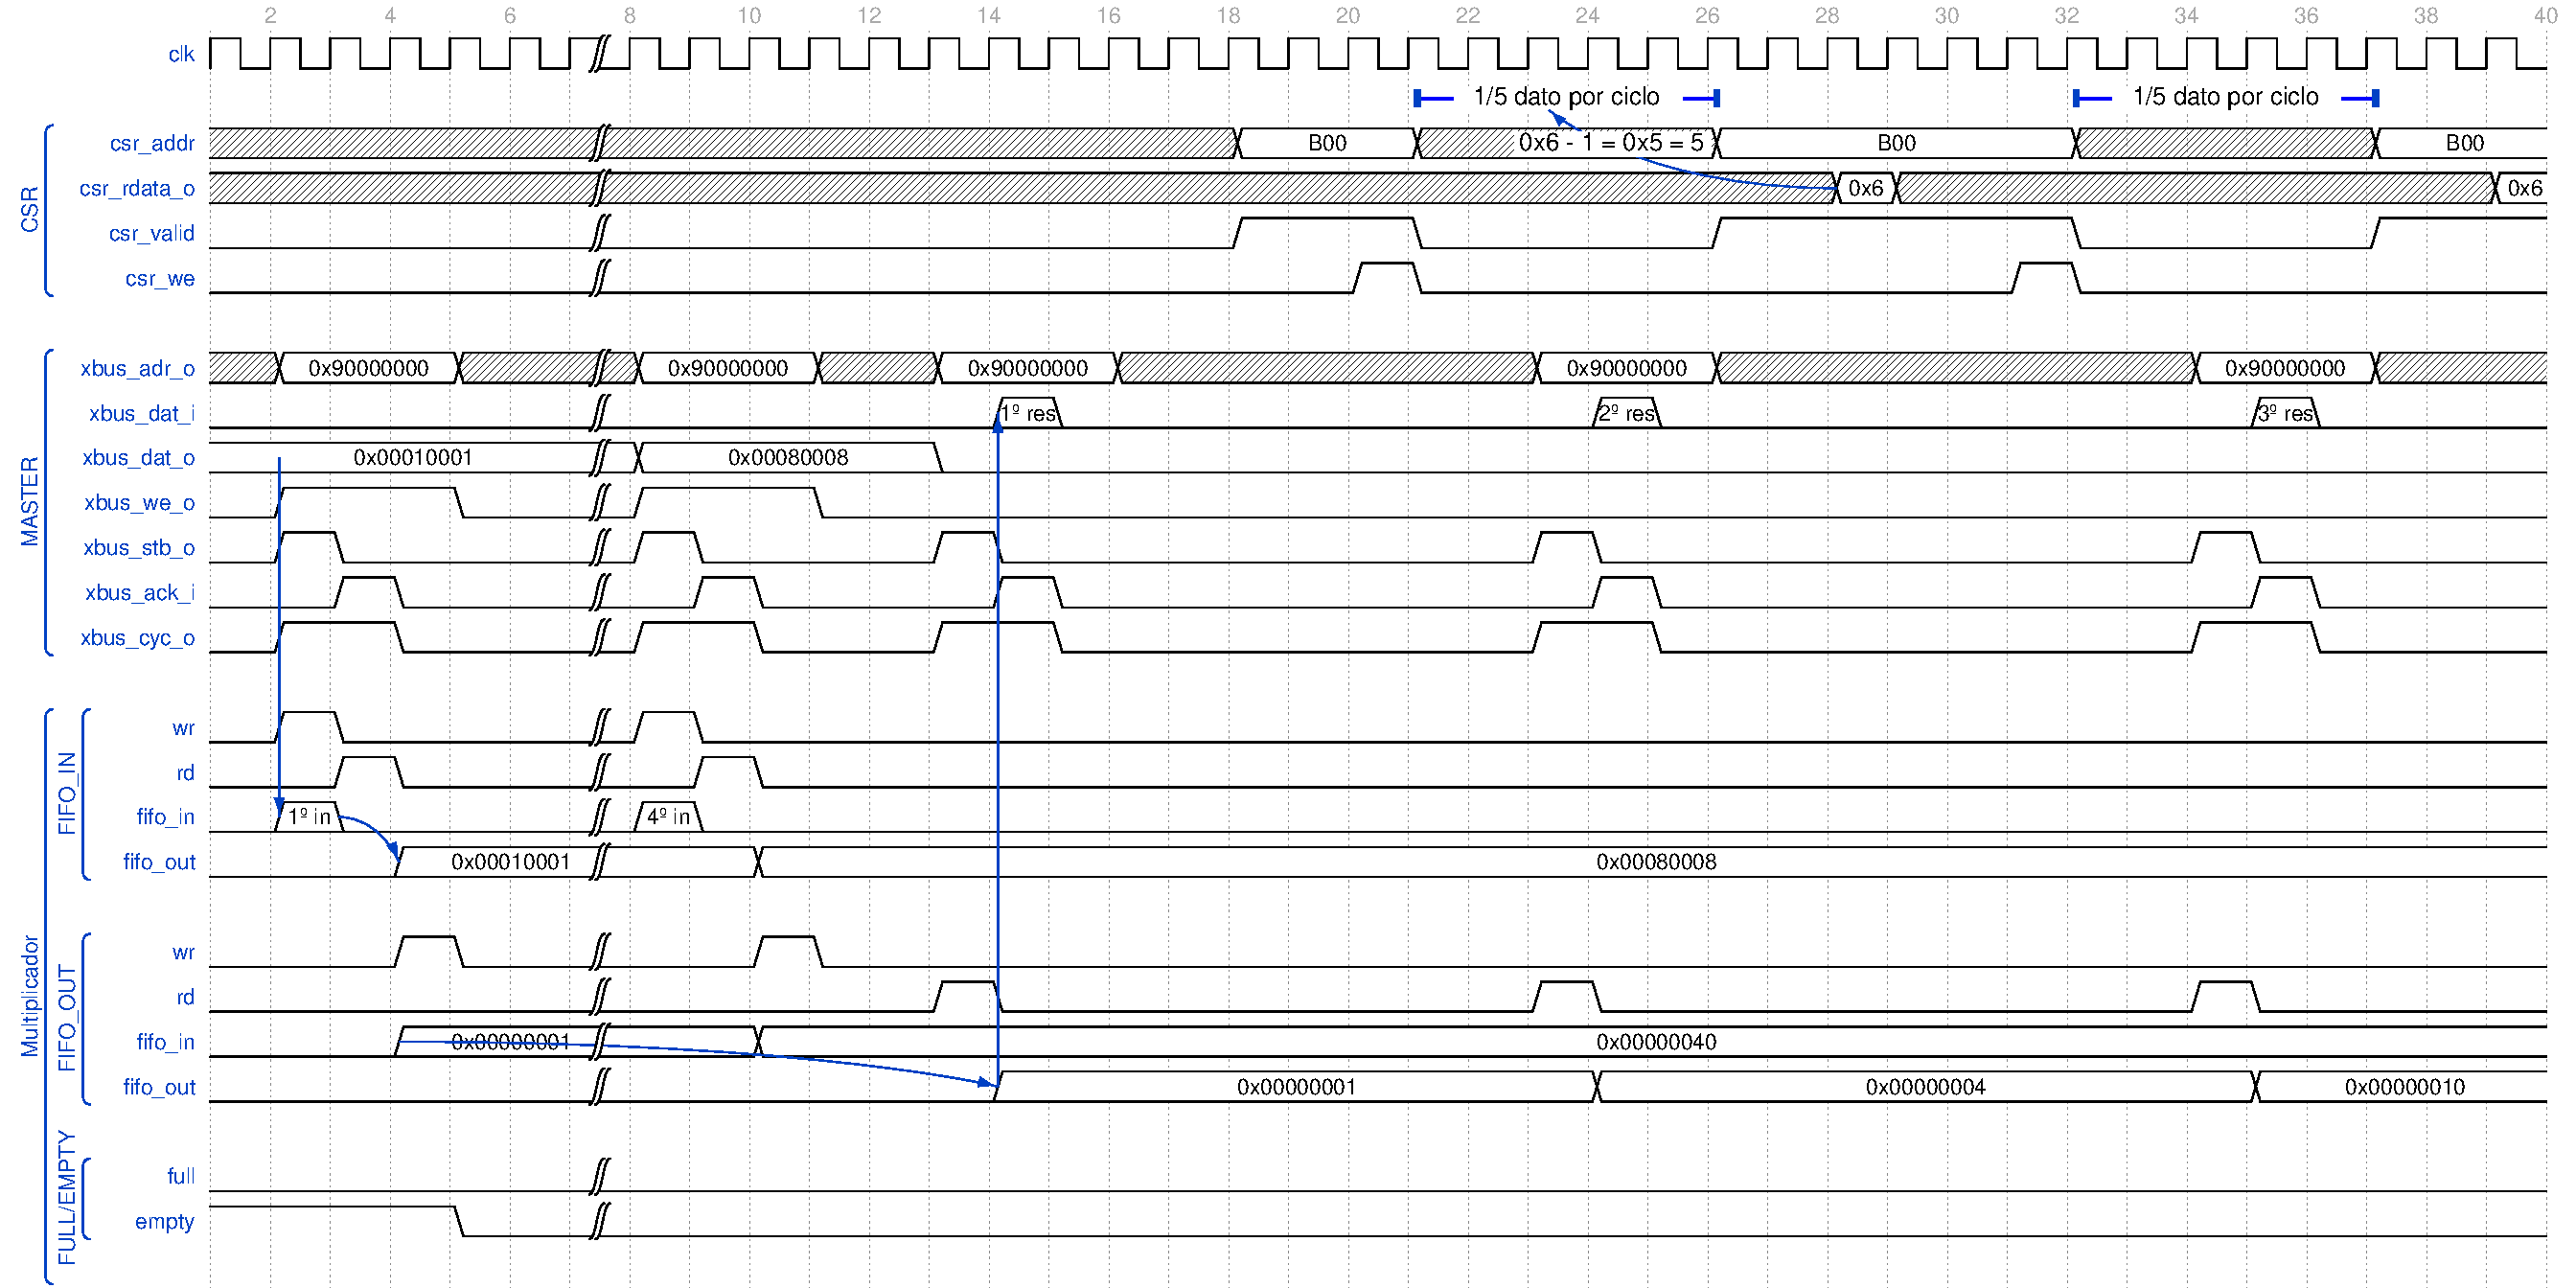
\includegraphics[width=17cm,angle=90]{Figuras/wave-xbus.pdf}
    \caption{Forma de onda resultante del ensayo de \textit{throughput} para NEORV32 + Mult-BP acoplado mediante XBUS.}
    \label{wave:xbus}
\end{figure}

\newpage

\begin{figure}[h!]
    \centering
    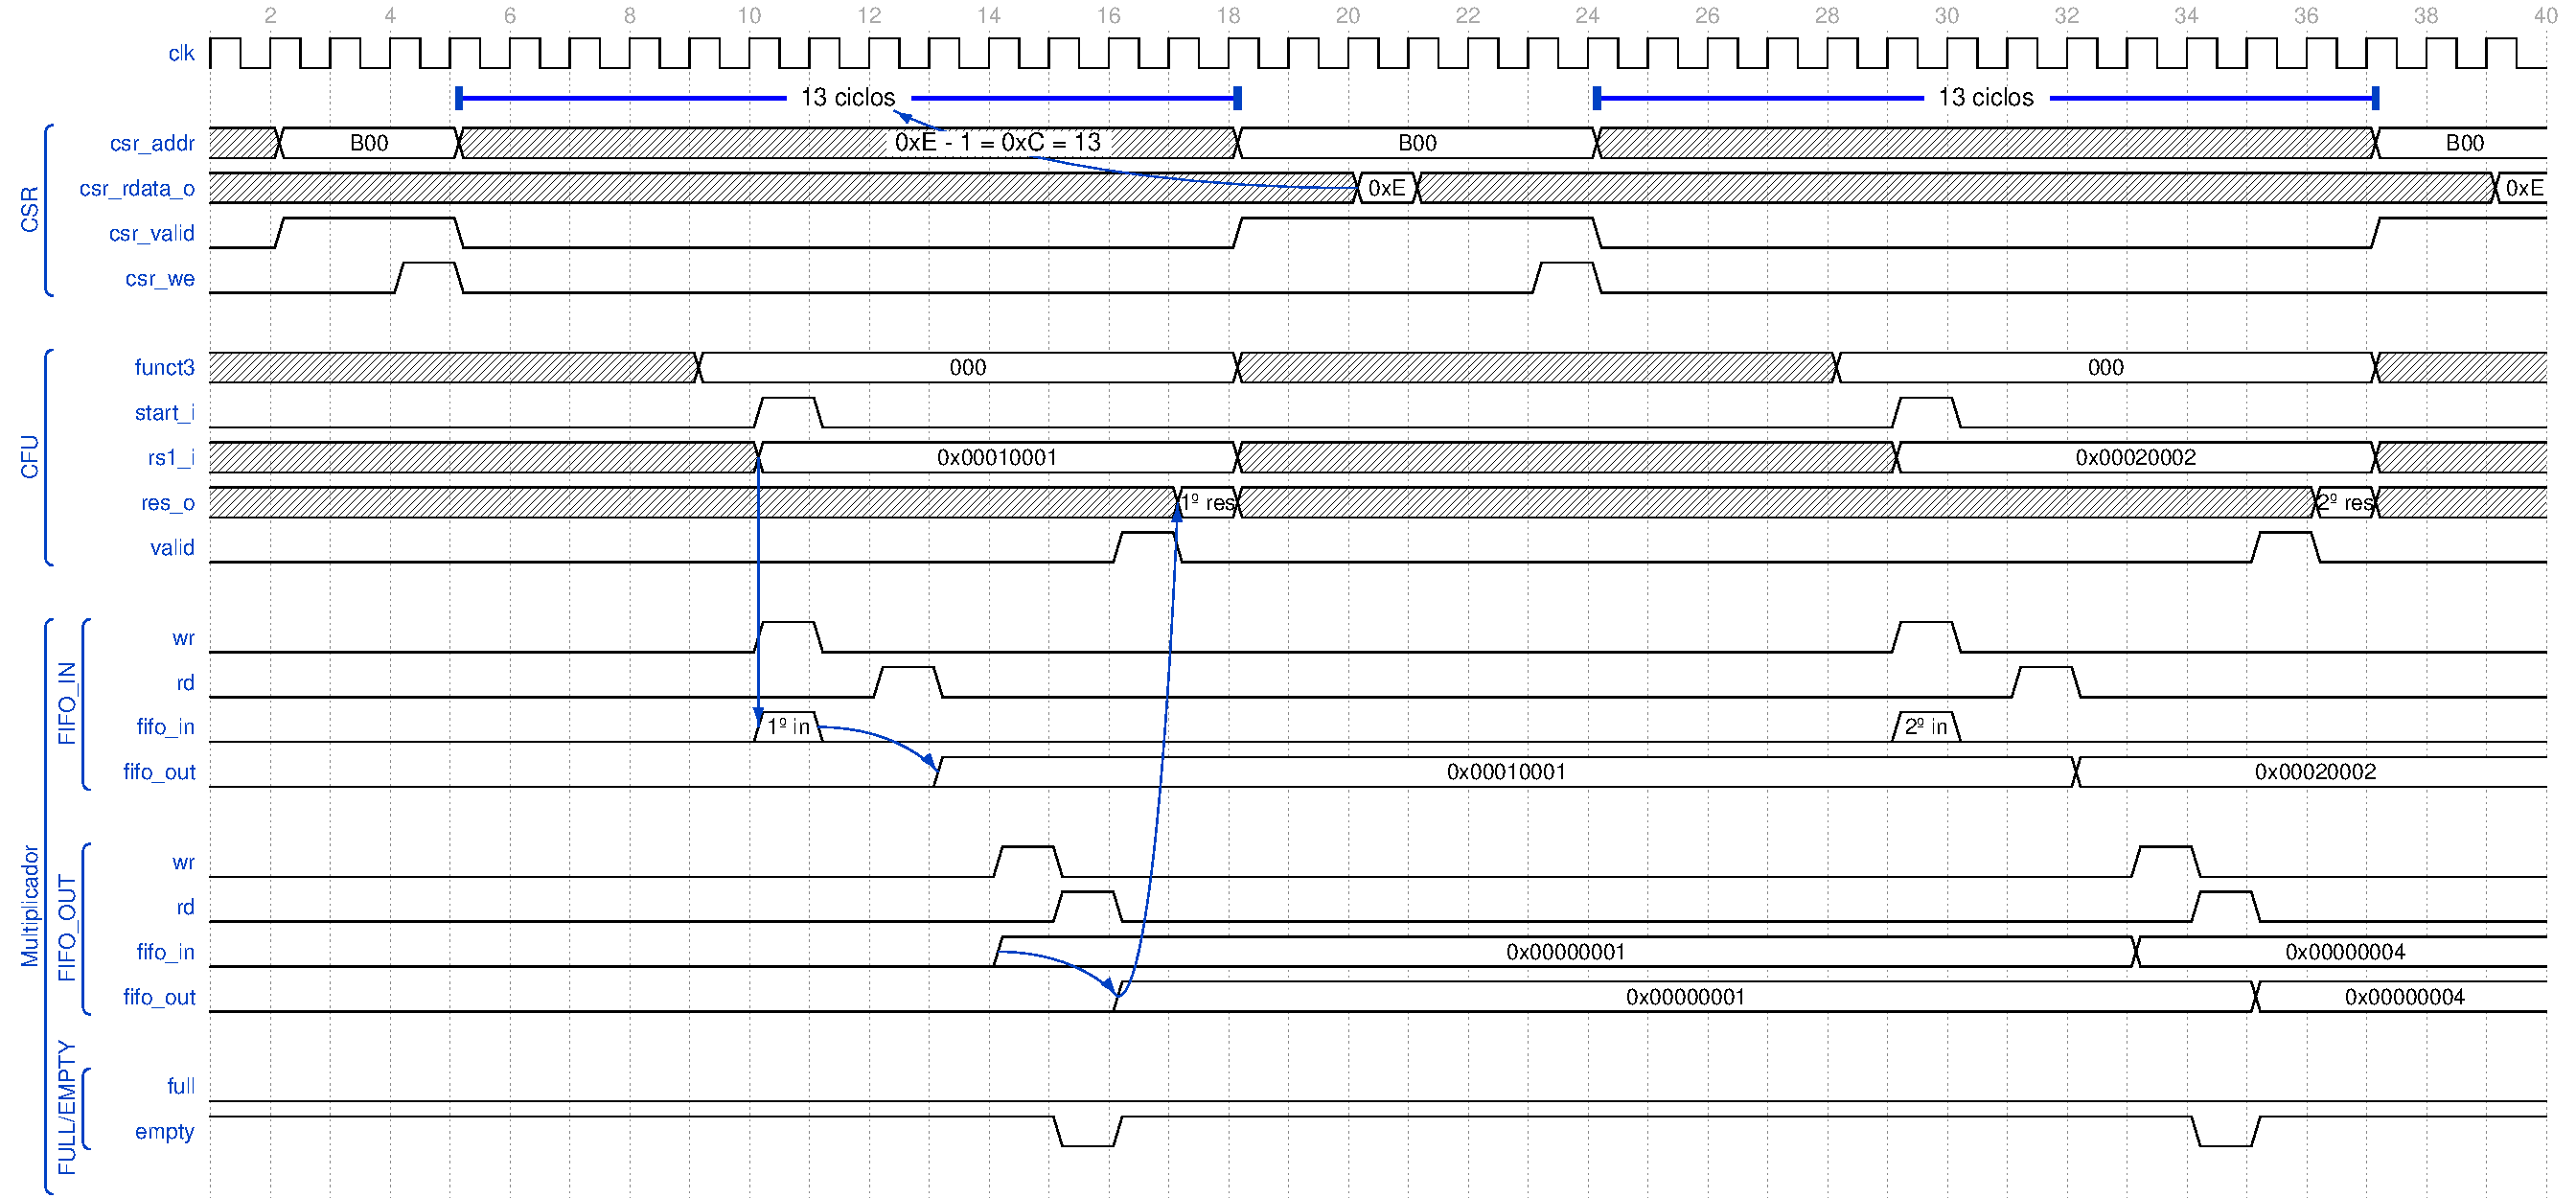
\includegraphics[width=22cm,angle=90]{Figuras/wave-cfu.pdf}
    \caption{Forma de onda resultante del ensayo de latencia para NEORV32 + Mult-B acoplado mediante CFU.}
    \label{wave:cfu}
\end{figure}

\newpage

\begin{figure}[h!]
    \centering
    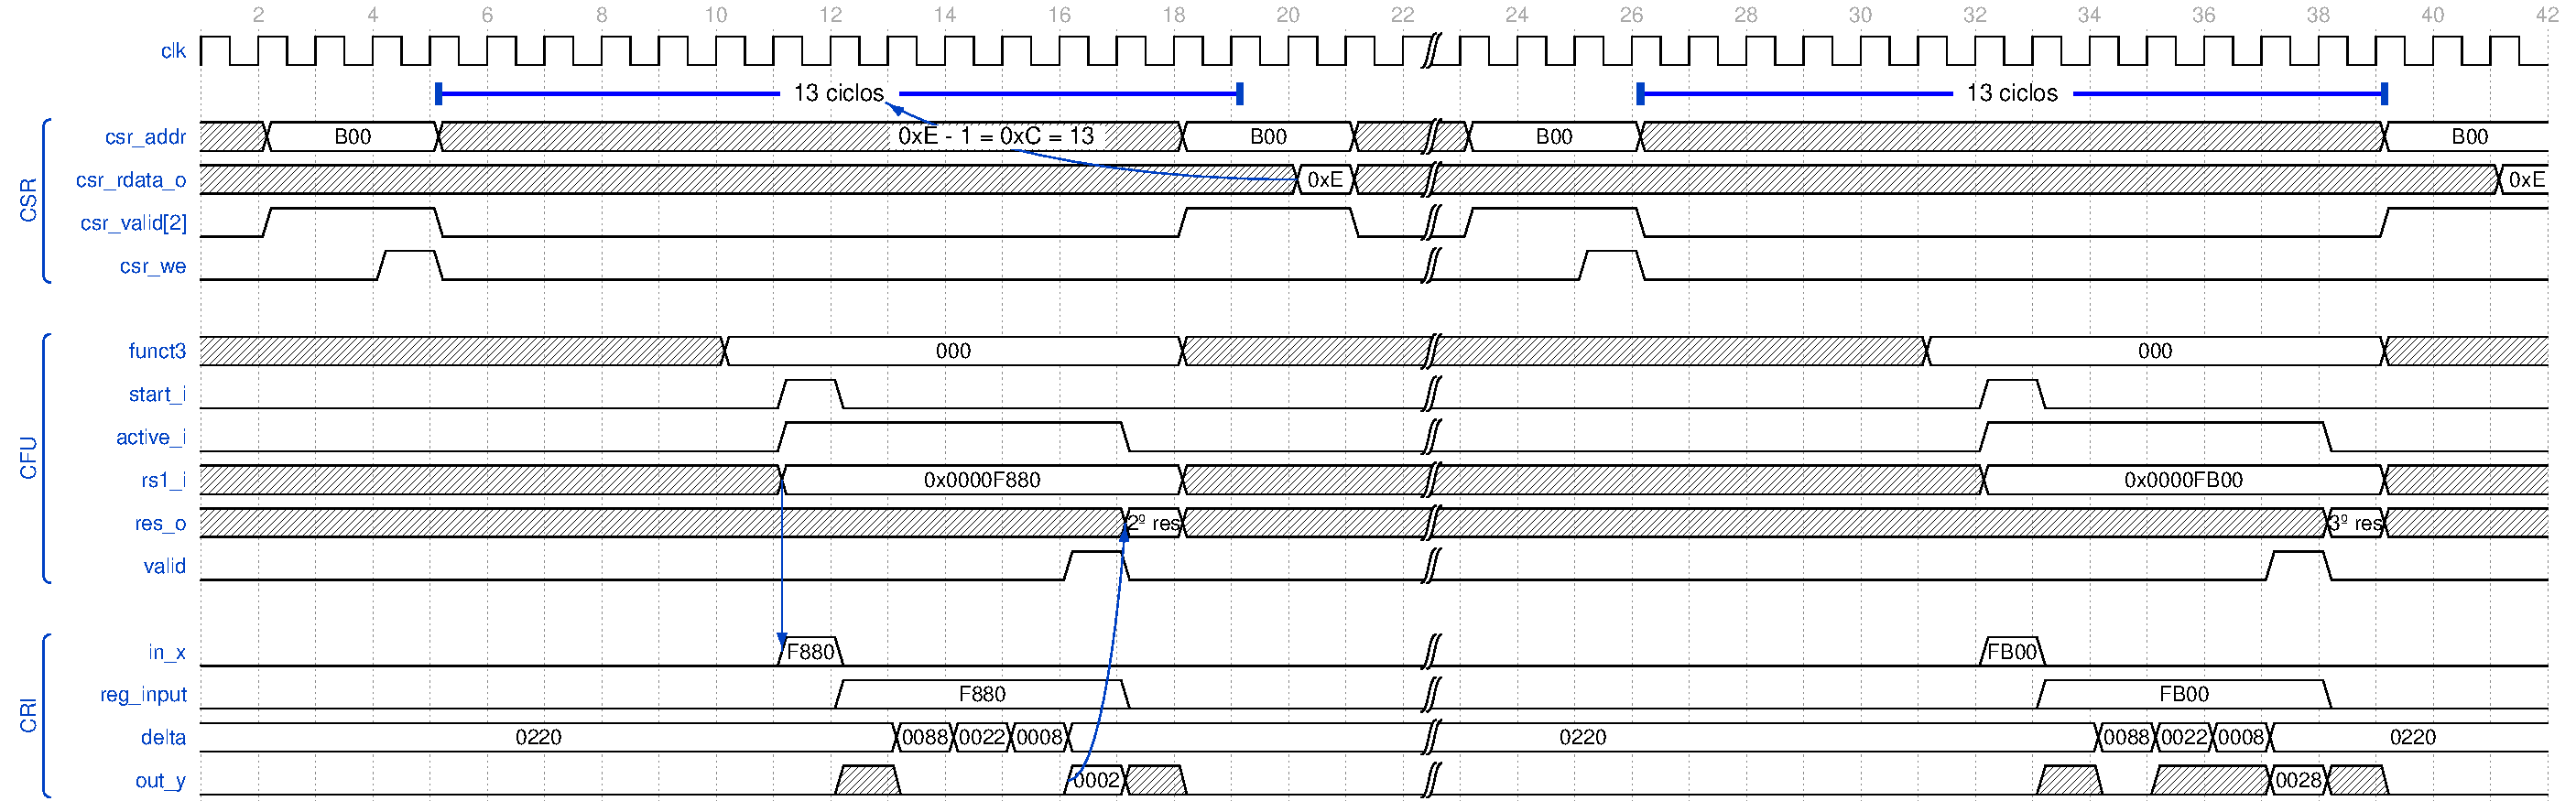
\includegraphics[width=22cm,angle=90]{Figuras/wave-sig.pdf}
    \caption{Forma de onda resultante del cálculo de dos sigmoides mediante CRI acoplado vía CFU con el NEORV32.}
    \label{wave:sig}
\end{figure}
